% CONTINUE ITALICS

\documentclass[11.5pt]{sig-alternate} % sets document style to sig-alternate
% packages
% typesetting
%\usepackage{dirtytalk} % typset quotations easier (\say{stuff})
\usepackage{hanging} % hanging paragraphs
\usepackage[defaultlines=3,all]{nowidow} % avoid widows
\usepackage[pdfpagelabels=false]{hyperref} % produce hypertext links, includes backref and nameref
\usepackage{xurl} % defines url linebreaks, loads url package
\usepackage{microtype}
\usepackage{textgreek}
%\usepackage{textcomp}
%\newcommand{\texttildemid}{\raisebox{0.4ex}{\texttildelow}}
% layout
\usepackage{enumitem} % control layout of itemize, enumerate, description
\usepackage{fancyhdr} % control page headers and footers
\usepackage{float} % improved interface for floating objects
%\usepackage{multicol} % intermix single and multiple column pages
% language
\usepackage[utf8]{inputenc} % accept different input encodings
\usepackage[english]{babel} % multilanguage support
% misc
\usepackage{graphicx} % builds upon graphics package, \includegraphics
%\usepackage{lastpage} % reference number of pages
%\usepackage{comment} % exclude portions of text (?)
\usepackage{xcolor} % color extensions
\usepackage[backend=biber, style=apa]{biblatex} % sophisticated bibliographies % necessary for HTML to display author info and date on abstract page
\usepackage{csquotes} % advanced quotations, makes biblatex happy
\usepackage{authblk} % support for footnote style author/affiliation
% tables and figures
\usepackage{tabularray}
%\usepackage{array} % extend array and tabular environments
\usepackage{caption} % customize captions in figures and tables (rotating captions, sideways captions, etc)
%\usepackage{cuted} % allow mixing of \onecolumn and \twocolumn on same page
\usepackage{multirow} % create tabular cells spanning multiple rows
%\usepackage{subfigure} % deprecated, support for manipulation of small figures
%\usepackage{tabularx} % extension of tabular with column designator "x", creates paragraph-like column whose width automatically expands
%\usepackage{wrapfig} % allows figures or tables to have text wrapped around them
%\usepackage{booktabs} % better rules
% dummy text
%\usepackage{blindtext} % blind text dummy text
%\usepackage{kantlipsum} % Kant style dummy text
\usepackage{lipsum} %lorem ipsum dummy text
% other helpful packages may be booktabs, longtable, longtabu, microtype

\pagestyle{fancy} % sets pagestyle to fancy for fancy headers and footers

% header and footer
% modern way to set header image
\renewcommand{\headrulewidth}{0pt} % defines thickness of line under header
\renewcommand{\footrulewidth}{0pt} % defines thickness of line above header
\setlength\headheight{80.0pt} % sets height between top margin and header image, effectively moves page contents down
\addtolength{\textheight}{-80.0pt} % seems to affect the lower height. maybe only works properly if footer numbers enabled?
\fancyhf{}
\fancyhead[CE, CO]{
\includegraphics[width=\textwidth]{headerImage.png}}
% footer
%\fancyfoot[LE,LO]{Article Title Here \\ DOI: }% left footer article title and doi
%\fancyfoot[CE,CO]{{}} % center footer empty
%\fancyfoot[RE,RO]{\thepage} % right footer page numbers
%\pagenumbering{arabic} % arabic (1, 2, 3) numbering in footer

\hypersetup{colorlinks=true,urlcolor=blue} % sets link color to blue
\urlstyle{same} % sets url typeface to same as rest of text

% set caption and figure to italics, label bold, left align captions, does not transfer to HTML
\captionsetup{labelfont=bf, font={large, it}, justification=raggedright, singlelinecheck=false}
\renewcommand\theContinuedFloat{\alph{ContinuedFloat}}

%this next bit is confusing, but essentially changes the width of the abstract. Seems to have been copied from this https://tex.stackexchange.com/questions/151583/how-to-adjust-the-width-of-abstract
\let\oldabstract\abstract
\let\oldendabstract\endabstract
\makeatletter %changes @ catcode to enable modification (in parsep)
\renewenvironment{abstract} %alters the abstract environment
{\renewenvironment{quotation}%
               {\list{}{\addtolength{\leftmargin}{1em} % change this value to add or remove length to the the default ?
                        \listparindent 1.5em%
                        \itemindent    \listparindent%
                        \rightmargin   \leftmargin%
                        \parsep        \z@ \@plus\p@}%
                \item\relax}%
               {\endlist}%
\oldabstract}
{\oldendabstract}
\makeatother %changes @ catcode to disable modification

% checks
% italics
% links -
% dashes -
% tildes
\begin{document}

\title{Gender Differences in Perceived Value of a Program to Promote Academic and Career Success for Students with Disabilities}

\author[1]{\large \color{blue}Sheryl Burgstahler }
\author[2]{\large \color{blue}Chuan Chang }

\affil[1]{University of Washington}
\affil[2]{University of Hawaii at Manoa}

\toappear{}
%% ABSTRACT
\maketitle
\begin{@twocolumnfalse} 
\begin{abstract}
\item 
\textit{This article reports the results of a retrospective survey of participants in an exemplary transition program for college-bound youth with disabilities. The study compared how male and female participants perceived changes in themselves in the areas of academic skills, social skills, Internet skills, levels of preparation for college and employment, levels of awareness of career options, and personal characteristics during the course of their participation; values of program components; and impact of program participation on their lives. In accordance with conventional gender stereotypes, significantly more boys indicated initial interests and/or career goals in the fields of science, technology, engineering, and mathematics (STEM). Financial security was reported by significantly more males and pursuit of independent living by significantly more females when asked about their primary motivation for seeking employment. Females perceived significantly greater changes in themselves than did males during the course of their participation. Girls reported that, prior to program participation, they perceived fewer career options than boys; by the time of the survey, females perceived more career options than males. Research results are of particular relevance to the preparation of girls with disabilities for college and careers, particularly in fields where they have been underrepresented.}
\\ \\
     
\end{abstract}
\end{@twocolumnfalse}

%% AUTHOR INFORMATION

\textbf{*Corresponding Author, Sheryl Burgstahler }\\
\href{mailto: sherylb@u.washington.edu  }{(sherylb@u.washington.edu )} \\
\textit{Submitted  Apr 14 2014}\\
\textit{Accepted Apr 14 2014} \\
\textit{Published online Apr 14 2014} \\
\textit{DOI:10.14448/jsesd.01.0001} \\
\pagebreak
\clearpage
\begin{large}
\section*{INTRODUCTION}
 
Individuals with disabilities are far less successful in school and employment than their peers without disabilities (Benz, Doren, \& Yavonoff, 1998; McNeil, 1997; National Organization on Disability, 2004). As high school support systems cease after graduation, many students with disabilities lack the selfdetermination, academic, transition, and independent living skills to succeed in college and careers. Consequently, fewer students with disabilities enroll and persist in postsecondary institutions than their peers without disabilities (Henderson, 2001; National Council on Disability and Social Security Administration, 2000; National Organization on Disability, 2004; Wagner, Newman, Cameto, \& Levine, 2005). This situation limits the success of people with disabilities in a world where completion of a postsecondary education is required for many lucrative careers.  
 
\section*{INDIVIDUALS WITH DISABILITIES AND STEM}
 
Individuals with disabilities are underrepresented in postsecondary studies and careers in science, technology, engineering, and mathematics (STEM) (National Science Foundation, 2000, 2007; Office of Disability Employment Policy, 2001). Factors that have been identified as contributing to the underrepresentation of individuals with disabilities in STEM fields include: 
 
\begin{itemize}
    \item 	little access to positive role models with disabilities in STEM fields (National organization on Disability, 2004; Seymour \& Hunter, 1998);
    \item 	social isolation from peers (Seymour \& Hun\-ter, 1998; Smith \& Nelson, 1993);
    \item 	low expectations and lack of encouragement from educators, counselors, parents, and others with whom they interact (National Science Foundation, 2000; Seymour \& Hunter, 1998; Task Force on Women, Minorities, and the Handicapped in Science and Technology, 1989);
    \item lack of knowledge about the content and requirements of STEM fields on the part of students with disabilities, counselors, social services staff, and special education teachers (Skolnick, Langbort, \& Day, 1982);
    \item 	inaccessible facilities, curriculum materials, equipment, and electronic resources (National Center for Education Statistics, 2000b; National Science Foundation, 2006);
    \item 	inadequate academic supports to bridge pre-college, college, and employment; and
    \item lack of understanding about effective accommodations on the part of students with disabilities and educators (Brazier, Parry, \& Fischbach, 2000; Heidare, 1996;Presidential Task Force on Employment of Adults with Disabilities, 1999; Task Force on Women, Minorities, and the Handicapped in Science and Technology, 1989; Womble \& Walker, 2001).
\end{itemize}
 
Career achievements of some people with disabilities suggest that there is potential to increase their representation in STEM fields (Blumenkopf, Stern, Swanson, \& Wohlers, 1996; DO-IT, 2006; Unger, Wehman, Yasuda, Campbell, \& Green, 2001). High-tech careers are particularly accessible to individuals with disabilities because of advances in assistive technology that provide access to computers and scientific equipment. However, the inaccessible design of software, web pages, distance learning courses, and facilities continues to limit access to these fields (Burgstahler, 2002b; National Center for Education Statistics, 2000a, 2000b; Schmetzke, 2001). 
 
\section*{FEMALES AND STEM}
 
Although their participation is increasing (National Science Foundation, 2007), the proportion of women in STEM fields falls below that of men (Galpin, Sanders, Turner, \& Venter, 2003; National Science Foundation, 2007; vanLangen \& Dekkers, 2006). Factors identified as contributors to this gender underrepresentation include discrimination, social pressure from parents and peers, and internalized negative attitudes and beliefs about mathematics (European Commission, 2001; Roger \& Duffield, 2000; Steele, 1997; Watt, 2005). Sex role stereotyping promotes the notion that boys are inherently better at math and have more use for math skills than girls (e.g., Eccles, 1994). Even girls who do well in mathematics often rate their math ability lower than do boys who perform at the same level (Kaminski, Erickson, Ross, \& Bradfield, 1976; Levine, 1976). Lower levels of self-perceptions in regard to their own math talent and expectations for mathematical success have been identified as strong contributors to girls’ lower participation in math (Eccles, 1994).  
 
Research also suggests that women employed in STEM fields tend to experience gender discrimination that mirrors what is experienced in secondary and postsecondary school contexts (Kusk, Ozbilgin, \& Ozkale, 2007; Olubor, 2006).  Interestingly, it has been found that in some socialist and formerly communist nations, perhaps due to emphasis on economic/gender equity, greater percentages of women are involved in STEM professions (Hanson, Schaub, \& Baker, 1996; Hanson, Fuchs, Aisenbrey, \& Kravets, 1999). In more Westernized nations, however, acceptance of stereotypes of females as less competent than men in STEM and of STEM as “too difficult” for females limits their exploration of careers in these fields (Greenfield, Peters, Lane, Rees, \& Samuels, 
2002; Roger \& Duffield, 2000; Seymour \& Hewitt, 1997; Steele, 1997; Watt, 2005) and contributes to gender inequity within STEM careers (Bianchini, Cavazos, \& Helms, 2000; Gurer \& Camp, 2002).  
 
A number of researchers have reported that adolescent girls lack self-confidence (Josephs, Markus, \& Tafarodi, 1992; Stipek \& 
Gralinski, 1991; Takayoshi, Huot, \& Huot, 1999; Tenenbaum \& Leaper, 2003) and that lack of self-confidence is a driving force that leads many women to avoid male-dominated career fields (Gurer \& Camp, 2002). Other researchers have reported that relationships with others may be more central to the selfconcepts of women than of men (Miller, 1986; Roberts, 1991). Putting these together, the lack of availability of encouraging and supportive relationships or communities in STEM fields may have a disproportionately negative impact on women, as compared to men, who may have less need for this type of support yet more access to it (Bandalos, Yates, \& Thorndike-Christ, 1995; Gandhi, 2000).  
 
Evidence suggesting the decline of gender differences in quantitative skills is encouraging (Friedman, 1989; Hyde, Fennema, and Lamon, 1990; National Science Foundation, 2007; Pajares \& Miller, 1994; Stumpf \& Stanley, 1996). Clearly, differing math achievement does not explain gender differences in participation in fields that require math skills.  
 
\section*{PROMISING PRACTICES}
 
Various programs have identified promising practices for bringing underrepresented groups—racial/\\ethnic minorities, women, and people with disabilities—into STEM fields. These include (a) hands-on science experiences, (b) work-based learning and research experiences, (c) summer bridge programs between academic levels, and (d) peer and mentor support (Benz et al., 1998; Cohen \& Light, 2000; Doren \& Benz, 1998; Leyser, Vogel, \& Wyland, 1998; National Science Foundation, 2001, 2005; Phelps \& Hanley-Maxwell, 1997; Ulki-Steiner, KurtzCostes, \& Kinlaw, 2000). Comprehensive projects that integrate a variety of interventions have been found to be more successful in recruiting and retaining students with disabilities in STEM fields than isolated efforts (American Association for the Advancement of Science, 2001; National Science Foundation, 2005). One transition program that has implemented all of these strategies with students who have disabilities is the DO-IT Scholars program which is described in the next section. The research reported in this article compares the benefits of its specific interventions as perceived by female and male participants. 
 
\section*{THE DO-IT SCHOLARS PROGRAM}
 
The DO-IT Scholars program is hosted by the Disabilities, Opportunities, Internetworking, and Technology (DO-IT) Center at the University of Washington in Seattle. It was selected for exploration in the current study because it (a) serves students with a wide range of disabilities; (b) has well-defined components that lend themselves to comparative analysis; and (c) has characteristics of successful programs that include longevity, prestigious awards, sustained operations, positive evaluation data, attention in the press, and ongoing support from funding agencies (e.g., Closing the Gap, 1995; Marmer, 1995; Roos, 1994–1995). Moreover, as a result of support from the National Science Foundation, it has produced a large number of participants interested in STEM fields (Burgstahler \& Chang, in press; Kim-Rupnow \& Burgstahler, 2004). Figure 1 describes key components of the DO-IT Scholars program. 

\begin{figure}[h]
    \centering
    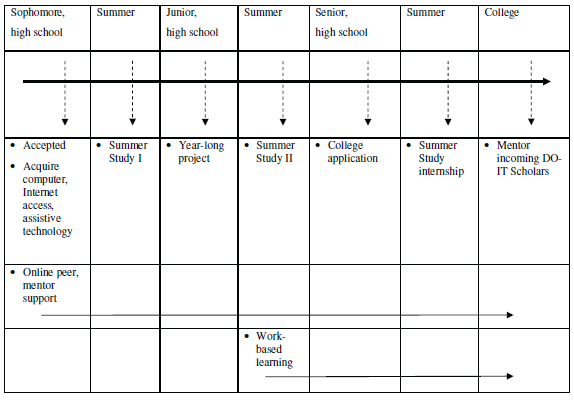
\includegraphics[width=1\linewidth]{fig1.png}
    \caption{Changes in self-rating scores regarding perceived career options over time by gender }
\end{figure}
 
\section*{INTERVENTIONS FOR DO-IT SCHOLARS }
 
DO-IT Scholars are college-bound high school students who face significant challenges to pursuing postsecondary studies and careers as a result of their disabilities. DO-IT activities are designed to help participants develop selfdetermination, social, academic, technology, and career skills. The program employs three primary interventions. Each offers activities in all fields of study and careers, but funding from the NSF has assured that opportunities to increase interests and skills in STEM are available throughout.  
 
\begin{itemize}
    \item 	Summer Study—Scholars participate in multiple residential programs at the University of Washington, where they are trained in computer and Internet use; socialize with other young people with disabilities; and prepare for college, careers, and independent living.
    \item 	Year-round computer and Internet activities—Computer and Internet skills continue to develop year-round in support of academic and career development and facilitate communication with mentors and peers.
    \item 	Work experiences—Internships and other work-based learning activities provide opportunities to explore interests, develop skills, practice disclosing disabilities,request accommodations, use technology, and learn to work with supervisors and coworkers.
\end{itemize}
 
\section*{PREVIOUS STUDIES OF THE DO-IT INTERVENTIONS }
 
Relevant findings of previous studies of DOIT interventions are summarized below. 
 
\begin{itemize}
    \item 	\textit{Parents} of DO-IT Scholars reported that DO-IT increased their children’s interest in college; awareness of career options; selfesteem; and self-advocacy, social, academic, and career/employment skills (Burgstahler, 2002a).
    \item 	\textit{DO-IT Mentors} reported discussing, STEM, college issues, disability-related issues, careers, computers, assistive technology, and the Internet with Scholars and expressed enjoyment in being there to help (Burgstahler \& Cronheim, 2001).
    \item 	\textit{DO-IT Scholars} reported that DO-IT participation helped them prepare for college and employment; develop Internet, self-ad\-vocacy, computer, social, and independent living skills; increase awareness of career options; and build selfesteem and perseverance (Burg\-stahler, 2003; Kim-Rupnow \& Burgstahler, 2004).
    \item 	Scholars reported the greatest effects of the Summer Study to be the development of social skills, followed by academic and career skills; and the greatest effects of the year-round computer and Internet activities to be the development of career skills, followed by academic and social skills (Burgstahler, 2003; Kim-Rupnow \&Burgstahler, 2004). Results suggest that DO-IT may increase the STEM interests of individuals not initially interested in STEM, but that these individuals tend to value social opportunities more highly than those with STEM interests, who are more interested in technology-related activities. (Burgstahler \& Chang, in press).
    \item 	Those who participated in work-based learning opportunities reported increased motivation to work toward a career, knowledge about careers and the workplace, job skills, ability to work with supervisors and coworkers, and skills in self-advocating for accommodations (Burgstahler, 2001; Burgstahler, Bellman, \& Lopez, 2004).
    \item 	Scholars in focus groups reported positive aspects of email communication to include being able get multiple answers to questions; meet people from around the world; and communicate quickly, easily, inexpensively, and independently with many people at one time (Burgstahler \& Cronheim, 2001; Burgstahler \& Doyle,2005). They predicted that access to the Internet and peer/mentor relationships would contribute to college and career (Burgstahler, 2003; Burgstahler \& Cronheim, 2001; Burgstahler \& Doyle, 2005; Kim-Rupnow \& Burgstahler, 2004). Most reported that DO-IT mentors stimulated interests in STEM.
    \item 	An analysis of the content of email messages revealed that male Scholars communicated more about the Internet and technology and females communicated more about personal matters, academic and career fields, career/volunteer work, disabilities, college transition, and DO-IT activities (Burgstahler \& Doyle, 2005).
\end{itemize}
 
\section*{RESEARCH QUESTIONS}
 
Given gender differences uncovered in the review of literature and analysis of Scholar email messages (Burgstahler \& Doyle, 2005), the researchers of the current study set out to examine whether the benefits of DO-IT activities were perceived differently by male and female participants. With funding from the NSF, further analysis of the data collected in the retrospective survey of DO-IT Scholars (Burgstahler \& Chang, in press; Kim-Rupnow \& Burgstahler, 2004) was conducted to address the following research questions. 
 
\begin{enumerate}
    \item \textit{How do female and male participants compare regarding primary disability types, academic interests/strengths and/or career goals, primary areas of postsecondary study, and motivations for going to college and gaining employment?}
    \item H\textit{ow do male and female participants compare regarding perceived changes in themselves in the areas of academic skills, social skills, levels of preparation for college and employment, levels of awareness of career options, and personal characteristics such as perseverance and self-esteem during the course of their participation in the DO-IT Scholars program?}
    \item \textit{How do female and male participants compare regarding perceived value of program components and what they consider to be the greatest overall impact of DO-IT on their lives?}
\end{enumerate}
 
\section*{METHOD}
 
\subsection*{Participants}
 
A total of 75 DO-IT participants completed the survey instrument used in the reported study (Kim-Rupnow \& Burgstahler, 2004). This final sample consisted of almost even numbers of male (52\%) and female (48\%) participants who were up to 26 years old (with 81\% of age 18-23). Forty-two percent of the participants indicated a mobility/orthopedic impairment as their primary disability; the rest of the sample was fairly evenly divided with respect to sight, hearing, learning, and other disabilities. Ninety-one percent of the participants had graduated from high school at the time the survey was conducted. A profile of the participants is shown in Table 1.  

\begin{table}[th]
\caption{Demographic Description of the Survey Respondents}
\begin{tabular}{llll}
\hline
Category & N & & \% \\ \hline
Gender & 75 & & \\
\hspace{1em} Male & & 39 & 52\% \\
\hspace{1em} Female & & 36 & 48\% \\ \hline
Age & 75 & & \\
\hspace{1em} Under 18 & & 1 & 1\% \\
\hspace{1em} 18–20 & & 6 & 8\% \\
\hspace{1em} 21–23 & & 35 & 47\% \\
\hspace{1em} 24–26 & & 25 & 33\% \\
\hspace{1em} Over 26 & & 8 & 11\% \\ \hline
Primary disability & 74 & & \\
\hspace{1em} Mobility & & 31 & 42\% \\
\hspace{1em} Sight & & 10 & 13.5\% \\
\hspace{1em} Learning & & 9 & 12\% \\
\hspace{1em} Hearing/Speech & & 7 & 9.5\% \\
\hspace{1em} Other & & 17 & 23\% \\ \hline
Graduated from high school? & 74 & & \\
\hspace{1em} Yes & & 67 & 91\% \\
\hspace{1em} No & & 7 & 10\% \\ \hline
\end{tabular}
\end{table}
 
The survey questionnaire created in an earlier study (Kim-Rupnow \& Burgstahler, 2004) included four sections: (a) demographic information, (b) Summer Study programs, (c) year-round computer and Internet activities, and (d) changes in Scholars as a result of participation. Demographic information collected ranged from age and gender to postsecondary education and employment (see Table 1). In the Summer Study section, respondents were asked to rate the value of program components such as college and career preparation on a scale ranging from 1 (not valuable at all) to 5 (extremely valuable). Using the same scale, in the year-round computer and Internet activities section, respondents were asked to rate the importance of activities such as online communication with peers and mentors; they also rated the value of both the Summer Study and yearround computer and Internet activities in developing their social, career, and academic skills. In the final section, respondents assessed their level of specific skills (e.g., selfadvocacy) at three different points in their lives–before participating in DO-IT, after the first Summer Study, and at the time of the survey. Statistical analyses provided both descriptive statistics—including frequency, cross-tabulation, and means—as well as inferential statistics, including Pearson’s Chisquare test, independent-samples t test, and mixed two-way repeated measures analyses of variance tests. For open-ended survey items, content analyses were performed to find general patterns in the narrative. 
 
Of the 173 participants from 1993 to 2000, the 155 individuals for which DO-IT has contact information were sent an email message asking them to complete a web-based survey or, alternatively, to request an email version of the survey, and to give permission to include their responses in the study. Non-respondents were mailed a follow-up printed survey and a postage-paid return envelope. Seventy-five Scholars responded to the questionnaire (44 via web-based questionnaire, 3 via email, and 28 via postal mail), resulting in a 48\% response rate.  
 
\section*{RESULTS}
 
Results are organized by research question in the following paragraphs. 
 
\textit{Research Question 1: How do female and male participants compare regarding primary disability types, academic interests/strengths and/or career goals, primary areas of postsecondary study, and motivations for going to college and gaining employment?}
 
\textbf{Primary disability type}s. Information about participants’ primary disabilities was coded into five categories: mobility/orthopedic, sight, hearing/speech, learning, and other. Table 2 shows the distribution patterns for the male and female participants. The patterns were similar between genders, with a disability related to mobility being the most common type of disability for both genders. Because of the low prevalence of types of disabilities other than mobility, these data were dichotomized (mobility vs. non-mobility disabilities) for analysis with Pearson’s Chisquare test. The test revealed no significant association between the type of disability and gender.  

\begin{table*}[ht]
\caption{Percentages (Numbers) of Responses Regarding Disability, Academic Strength \& Career Goal, and Area of Postsecondary Study, by Gender}
\begin{tabular}{lll}
\hline
Category & Male & Female \\ \hline
Primary disability & & \\   
\hspace{2em} Mobility & 35.9\% (14) & 51.4\% (18) \\
\hspace{2em} Sight & 17.9\% (7) & 8.6\% (3) \\
\hspace{2em} Hearing/Speech & 7.7\% (3) & 11.4\% (4) \\
\hspace{2em} Learning & 15.4\% (6) & 8.6\% (3) \\
\hspace{2em} Other & 23.1\% (9) & 20.0\% (7) \\
Primary disability (dichotomized) & & \\
\hspace{2em} Mobility & 35.9\% (14) & 51.4\% (18) \\
\hspace{2em} Non-mobility & 64.1\% (25) & 48.6\% (17) \\
Academic strength/career goal & & \\
\hspace{2em} STEM & 61.5\% (24) & 38.2\% (13) \\
\hspace{2em} Non-STEM & 38.5\% (15) & 61.8\% (21) \\
Area of postsecondary study (unclassified omitted) & & \\
\hspace{2em} STEM-related & 70.0\% (21) & 46.4\% (13) \\
\hspace{2em} Liberal/General & 30.0\% ( 9) & 53.6\% (15) \\ \hline
\end{tabular}
\end{table*}
 
\textbf{Academic interests/strengths and/or career goals}. Two categories were identified based on participant responses to questions about academic interests/strengths and career goals. Participants who reported having interests/strengths and/or career goals in science, technology, engineering, or mathematics (STEM) fields were coded as members of the STEM-oriented group and the rest of the participants were coded into the non-STEM group. As indicated in Table 2, sixty-two percent of the male participants expressed interests/strengths and or career goals in STEM. In contrast, only 38\% of the female participants were STEM-oriented. Pearson’s Chi-square test confirms that this disproportionality is unlikely due to a chance distribution of males and females into the two groups, \textchi\textsuperscript{2}(1, \textit{N} = 73) = 3.95, \textit{p} < .05; significantly more males expressed interests/strengths and/or career goals in STEM fields and significantly more females expressed interests/strengths and/or career goals in non-STEM field 
 
\textbf{Primary areas of postsecondary study}. Reported areas of postsecondary study were coded into three categories: STEM, liberal/general, and undecided/unclassified. Table 2 shows that a majority of the male respondents (70\%) chose to study in STEM related majors, however, the female respondents split almost equally between STEM and non-STEM-oriented majors, with 46\% and 54\% of them in STEM and liberal/gen\-eral fields, respectively. Because of the low prevalence of unclassified students (3 in total), this category was omitted from analysis with Pearson’s Chi-square test. The difference between males and females in their choices of majors approached significance at the .05 level, \textchi\textsuperscript{2}(1, \textit{N} = 58) = 3.32, \textit{p} = 0.07. 

\textbf{Motivation for employment}. Responses to an open-ended question about primary motivations for gaining employment were coded into 5 categories: Pursuit of independent living, financial security/incentive plan, contribution to social change, helping others, and other. Examination of Table 3 reveals that pursuit of independent living and financial security were the most frequently reported motivators for seeking employment by both genders. Because of the low prevalence in contribution to social changes, helping others, and other categories, they were omitted from analysis with Pearson’s Chi-square test. The analysis revealed significant gender differences in response patterns, \textchi\textsuperscript{2}(1, \textit{N} = 53) = 6.94, \textit{p} < .01, with financial security being reported by significantly more of the male participants and pursuit of independent living being reported by significantly more of the female participants. 

\begin{table*}[th]
\caption{Percentages (Numbers) of Responses Regarding Primary Motivation for Employment, by Gender}
\begin{tabular}{lll}
\hline
Category & Male & Female \\ \hline
Primary motivation for employment & & \\
\hspace{2em} Pursuit of independent living & 21.9\% (7) & 56.7\% (17) \\
\hspace{2em} Financial security/Incentive plan & 59.4\% (19) & 33.3\% (10) \\
\hspace{2em} Contribution to social change & 3.1\% (1) & 0.0\% (0) \\
\hspace{2em} Helping others & 6.3\% (2) & 3.3\% (1) \\
\hspace{2em} Other & 9.4\% (3) & 6.7\% (2) \\ \hline
\end{tabular}
\end{table*}
 
\textit{Research Question 2: How do male and female participants compare regarding perceived changes in themselves in the areas of academic skills, social skills, levels of preparation for college and employment, levels of awareness of career options, selfesteem, and personal characteristics such as perseverance during the course of their participation in the DO-IT Scholars program? }
 
DO-IT Scholars were asked to assess their academic skills, social skills, levels of preparation for college and employment, levels of awareness of career options, and personal characteristics such as perseverance and self-esteem at three points: prior to their involvement in DO-IT (Phase 1), immediately following their first DO-IT Summer Study (Phase 2), and at the time of the current survey (Phase 3). Information on the first two phases was retrospective in that survey participants were asked to recall and rate themselves at each of two earlier points in time.  
 
Average change scores were created by computing the difference between self-ratings provided at Time 3 and Time 1. For both genders the greatest positive changes reported were in the area of college preparation, with an average of 2.25 and 2.06 units of increase in male and female participants, respectively. The least improved area reported was perseverance, where an average of 0.85 and 0.94 units of increase in males and females were observed. Female participants reported higher positive changes on more self-rated areas than did their male counterparts. For example, while boys tended to report small changes in perceived career options, selfesteem, social skills, and perseverance, with the average scores of change from the baseline to follow-up less than 1, girls reported an increase of less than one unit only in the area of perseverance. 
 
To further examine the role of gender in how participants perceive the benefit of DO-IT interventions over time, multiple 2 x 3 analyses of variance (ANOVA) with repeated measures were conducted in all areas of growth using gender as the between-group factor and the three time points (phase) as the within-group factor. In the area of perceived career options, the analysis revealed a significant overall effect of time, meaning that as a group the DO-IT participants were increasingly positive about the impact of DOIT activities on their perception of career options as their involvement in these activities progressed. However, the significant group by time interaction indicates that the growth in this perception was different for young men and young women participants (\textit{F}(2, 63) = 5.80, \textit{p} < .01). Corresponding to this significant interaction effect, Figure 2 reveals a steeper increase in the perceived benefits of DO-IT activities among the young women than the young men. Analyses of the linear and quadratic components of this interaction show a significant linear component (\textit{F}(1, 64) = 7.01, \textit{p} < .01), but no significant quadratic component. Thus, there is a linear relationship between exposure to DO-IT activities and perception of benefits: the longer the exposure, the more positive the perceived impact. 

\begin{figure}[h]
    \centering
    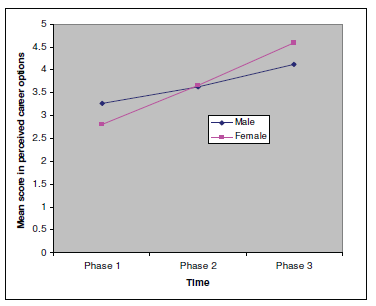
\includegraphics[width=1\linewidth]{fig2.png}
    \caption{Changes in self-rating scores regarding perceived career options over time by gender }
\end{figure}

Analysis of the simple main effect of time, holding gender constant, reveals that both male and female participants perceived their career options to be significantly expanded as the program progressed (\textit{F}(2, 63) = 11.52, \textit{p} < .001 for males; \textit{F}(2, 63) = 43.93, \textit{p} < .001 for females). Analysis of simple main effect of gender, holding time constant, shows that young women entered the program with their perception of career options lower than did young men. While being exposed to DO-IT activities, the females’ perceptions of career options caught up with the males’ by the end of their first Summer Study and surpassed that of the men by the time the current survey was conducted (Phase 1: \textit{F}(1, 64) = 2.47, \textit{ns}; Phase 2: \textit{F}(1, 64) = 0.02, \textit{ns}; Phase 3: \textit{F}(1, 64) = 7.19, \textit{p} < .01).  
 
Analyses of these repeated measures ANOVA using a traditional univariate approach led to the same conclusions for each of these areas with one important exception. While the multivariate approach detected no significant interaction between gender and time in Internet skills (\textit{F}(2, 65) = 2.26; \textit{p} > .05), this interaction reached statistical significance when the more powerful univariate approach was used (\textit{F}(2, 132) = 3.35; \textit{p} < .05). Female scores increased from a mean of 2.39 at Phase 1 to 3.85 at Phase 2 to 4.60 at Phase 3, a 92\% increase between the first and the third time point, while the means of male participants increased from 2.92 to 3.87 to 4.51, a 54\% increase over the same time period. It is not clear from these analyses whether the pattern of change in response to Internet skills was different for females and males. But analysis of simple main effect of gender, holding time constant, reveals that the females entered the program with lower perceptions of Internet skills than did the males (\textit{F}(1, 68) = 3.76; \textit{p} = .057); this difference approached statistical significance at the .05 level. However, the perceptions of the females caught up by the end of their first Summer Study and continued to improve at the same rate as that of the males until the survey was administered (Phase 2: \textit{F}(1, 67) = .00, \textit{ns}; Phase3: \textit{F}(1, 69) = .12, \textit{ns}). 
 
Regarding computer skills, levels of preparation for college and employment, selfadvocacy skills, self-esteem, social skills, and independence, the main effect of phase was consistently significant, indicating that both male and female participants perceived themselves to improve significantly in these areas from Phase 1 to Phase 2 and Phase 2 to Phase 3. In no case was the main effect of gender or the interaction between gender and phase statistically significant, indicating that participants of both genders perceived that they improved similarly over time in these areas. 
 
\textit{Research Question 3: How do female and male participants compare regarding perceived value of program components and what they consider to be the greatest overall impact of DO-IT on their lives? }
 
The following sections compare males with females regarding perceived benefits of DOIT Summer Study, year-round computer and Internet activities, and the program overall. 
 
\textbf{Summer Study}. Participants were asked to rate the values of the following Summer Study activities on their personal, academic, and/or career development using a 5-point Likert scale: (a) computer and Internet use, (b) face-to-face interaction and developing relationships, (c) college preparation, (d) career preparation, and (e) internship at Summer Study. All of the activities were rated highly, with scores ranging from 3.83 to 4.35 for males and 3.76 to 4.37 for females. Out of all Summer Study activities, survey respondents rated computer and Internet use as the most valuable. Independent samples t tests revealed no gender differences, indicating that young women and men perceived the values of Summer Study activities similarly.  
 
\textbf{Year-round computer and Internet activities}. Year-round computer and Internet activities included (a) access to a computer at home, (b) access to assistive technology, (c) online communication with peers, (d) online communication with adult mentors, and (e) access to information and resources on the Internet. All of the activities were perceived to be valuable by participants of both genders, with mean scores ranging from 3.62 to 4.53 for males and 3.91 to 4.59 for females. Access to a home computer and to information and resources on the Internet received the highest ratings from participants of both genders. An analysis using an independent samples t test did not reveal differences by gender. Furthermore, responses of the two groups were similarly highly positive when participants were asked how valuable the overall Summer Study program and yearround computer and Internet activities were in developing social, academic, and career/employment skills. 
 
\textbf{Greatest overall impact of DO-IT}. Participant responses to an open-ended question about what has been the greatest impact of DO-IT on their lives clustered into two main areas: (a) individual psychosocial development and (b) readiness for college and career pursuits. Participants of both genders responded similarly with nearly equal proportions of males and females categorized in each area.  
 
\section*{DISCUSSION AND IMPLICATIONS FOR OTHER PROGRAMS }
 
The current study compares how male and female participants in the DO-IT Scholars program perceive themselves and the impact of program participation. In accordance with conventional gender stereotypes, significantly more males than females indicated initial interests/ strengths and/or career goals in STEM fields and more males than females chose STEM fields as primary areas for postsecondary study. Where\-as less than 40\% of females indicated initial academic interests/strengths and/or career goals in STEM fields, almost half of the young women reported majoring in STEM postsecondary studies. Although it is unknown what role program interventions might have played, this finding suggests that career decisions are subject to influences and change as young adults engage in new experiences. As indicated in the literature review, factors contributing to the underrepresentation of females in STEM careers include lack of awareness of specific careers and educational requirements involved in pursuing them. For example, mathematics skills are needed for work in many STEM-related areas (Skolnick, Langbort, \& Day, 1982) and performance tests, graduate school exams, and civil service exams include questions measuring math skills (Kaminski et al., 1976). Even though lack of career awareness affects students of both genders, girls often suffer greater negative consequences than do boys because they are more likely to steer away from mathematics, physics, and science courses in high school (Watt, 2005). Additionally, often girls do not choose STEM because they do not perceive it to be socially meaningful and hence consider it of less value than do boys (Eccles, 1994). Accordingly, it has been suggested that making explicit connections between STEM fields and social values could heighten girls’ interests (Shanahan, 2006; Watt, 2005). All DO-IT interventions present STEM fields as accessible and socially meaningful and, in doing so, the program may have an impact on girls’ perceptions of studying and working in STEM fields.  Girls reported fewer career options than boys prior to program participation; by the time of the survey, however, their perceived career options significantly increased and surpassed that of males, suggesting that the program may have impacted females more than males in this area. Such positive impact is also captured in qualitative data. For example, discoveries reported by females include “realizing that I had more career choices than I previously thought I had,” and “[DO-IT] showed me the career that I hope to go into.” Female participants also tended to perceive more improvement than did males in Internet skills, self-esteem, and social skills. Studies on gender equity in STEM education and careers often point out that girls and women face gender stereotyping with respect to STEM. For girls with disabilities, their own expectations and those of others regarding studying STEM may be even lower than for girls without disabilities since students with disabilities are less encouraged to pursue STEM than their peers without disabilities. Girls’ exposure to the engaging DO-IT program may stimulate self exploration and discovery. As one young woman reported, “I think the greatest impact [of DO-IT] for me is it [is] helping me to understand more about myself and the people in [the] real world. I have learned how to adapt to society without thinking that I am disable[d], I am useless.” Comments like this suggest that DO-IT participation may positively impact the self esteem of young women. DO-IT Scholars have credited the program with helping them gain a positive outlook on life and disabilities, and expand their social network. Similar program outcomes have been confirmed by parents (Burgstahler, 2002a) and suggest that the program may impact the overall wellbeing of participants. %remove space in interests/strengths
 
Males and females in the current study differed in primary motivators for seeking employment. While financial security was reported by significantly more male students, pursuit of independent living was reported by more females. The pattern of differences poses interesting questions as the link between gender and career motivators is likely to be mediated through other variables such as socially-defined gender roles. For example, in the current society it may be that males generally feel more pressure than females to secure respectable salaries in order to support themselves and/or their families. Results suggest the importance of helping students develop practical skills in independent living and employment that can bring financial security. 
 
\section*{LIMITATIONS OF THE STUDY AND RECOMMENDATIONS FOR FURTHER RESEARCH }
 
Since DO-IT Scholar participants were not randomly selected, caution should be exercised in generalizing the results of this study to other populations. DO-IT participants are college-bound teens with disabilities who are motivated to participate in an extracurricular technology, academic, and career program that encourages consideration of STEM fields and who have supportive adults to assist with the application process. Results of this study should be interpreted in light of limitations reported in the earlier study (Kim-Rupnow \& Burgstahler, 2004). 

Specifically, the response rate of the present study was 48\%; a larger sample would have provided more power for analyses with multiple subgroups. Also, the impact of program components was based on the retrospective self-reporting of survey respondents. Their perceptions may not accurately reflect the actual impact of specific interventions due to potentially skewed recalls and subjectivity of self-assessment. Quantitative measures at actual points in time might provide stronger evidence of impact.  
 
Current study results suggest important issues for further research. More longitudinal followup research on transition programs like DO-IT is needed since little of such data is currently available in published literature. Collection of data should occur at critical steps—such as before the Summer Study, immediately after the Summer Study, six months later, one year later, and several years later—in order to detect the long-term effect of program activities. A follow-up study could be designed to shed light on what interventions make some participants turn away from other interests and goals to pursue STEM studies and careers. Lastly, perspectives of parents, high school teachers, counselors, and program staff should be incorporated regarding program effectiveness.  
 
\section*{CONCLUSION }
 
The current study explored gender differences in participant perceptions of personal characteristics and of the value of transition program interventions. Females with disabilities tended to perceive greater and more pervasive changes in themselves when compared to males as their program involvement progressed. Their retrospective recollections of career options before participation were lower than those of males, however significantly greater levels of perceived career options were reported by women than men at the time of the survey, suggesting that program activities may have increased perceived career options for girls more than boys. Results also suggest that girls may benefit from interventions to prepare them for college and careers even more than boys and contributes to the body of evidence that supports the efficacy of interventions to increase the participation of women in STEM and other fields where they have been underrepresented. This study provides evidence-based direction to those seeking to enhance the academic and career selfconcepts, interests, and skills of women with disabilities, particularly in fields where they have been underrepresented. It suggests that when promoting STEM studies and careers for individuals with disabilities, programs should consider not only issues related to disability but also those related to gender.  
 
\section*{AUTHOR NOTES AND ACKNOWLEDGEMENTS}
 
 
Sheryl Burgstahler is the founder and director of DO-IT, Affiliate Associate Professor in the College of Education, and Director of Accessible Technology Services at the University of Washington. Chuan Chang is at the Center on Disability Studies, University of Hawaii at Manoa, and external evaluator of DO-IT activities. 
 
The DO-IT Scholars program has been funded by the National Science Foundation (grant numbers 9725110, 9800324, and 9550003) and the State of Washington. Preparation of this article was partially supported by grants from the U.S. Department of Education, the National Institute on Disability Rehabilitation Research, and the Office of Special Education Programs (grant \#H133B980043), as well as the Rehabilitation Services Administration (grant \#H235N-010014) and the National Science Foundation (cooperative agreement \#HRD0227995). The opinions expressed in this paper are those of the authors and do not necessarily reflect those of the funding agencies. Some of the content of this article has been adapted with permission from publications on the DO-IT website at \url{http://www.washington.edu/doit/}. 

\end{large}
\include{} 
\section*{REFERENCES}\par 

\leftskip 0.25in
\parindent -0.25in 

American Association for the Advancement of Science. (2001). \textit{In pursuit of a diverse science, technology, engineering, and mathematics workforce}. Washington, DC: Author. 
 
Bandalos, D. L., Yates, K., \& ThorndikeChrist, T. (1995). Effects of math self-concept, perceived self-efficacy, and attributions for failure and success on test anxiety. \textit{Journal of Educational Psychology, 87}, 611–623.  
 
Benz, M., Doren, B., \& Yavonoff, P. (1998). Crossing the great divide: Predicting productive engagement for young women with disabilities. \textit{Career Development for Exceptional Individuals, 21}(1), 3–16. 
 
Bianchini, J. S., Cavazos, L. M., \& Helms, J. V. (2000). From professional lives to inclusive practice: Science teachers and scientists' views of gender and ethnicity in science education. \textit{Journal of Research in Science Teaching, 37}(6), 511–547. 
 
Blumenkopf, T., Stern, V., Swanson, A., \& Wohlers, D. (Eds.). (1996). \textit{Working chemists with disabilities: Expanding opportunities in science}. Washington, DC: American Chemical Society Committee on Chemists with Disabilities.  
 
Brazier, M., Parry, M., \& Fischbach, E. (2000). Blind students: Facing challenges in a college physics course—Lev\-eling the playing field for the visually impaired. \textit{Journal of College Science Teaching, 30}(2), 114–116.  
 
Burgstahler, S. (2001). A collaborative model promotes career success for students with disabilities: How DO-IT does it. \textit{Journal of Vocational Rehabilitation, 16} (129), 1–7. 
 
Burgstahler, S. (2002a). The value of DO-IT to kids who did it! \textit{Exceptional Parent, 32}(11), 79–86.  
 
Burgstahler, S. (2002b). Universal design of distance learning. \textit{Information Technology and Disabilities, 8}(1). Retrieved December 1, 2007, from \url{http://www.rit.edu/~ea-si/itd/itdv08n1/burgstahler.htm}  
 
Burgstahler, S., Bellman, S., \& Lopez, S. (2004). Research to practice: DO-IT prepares students with disabilities for employment. \textit{NACE Journal, 65}(1). Retrieved December 1, 2007, from \url{http://www.naceweb.org/Forms-Login.asp?/pubs/journal/fa04/bellman.htm}
 
Burgstahler, S. \& Chang, C. (in press). Promising interventions for promoting STEM fields to students who have disabilities. 
\textit{Review of Disability Studies}. 
 
Burgstahler, S., \& Cronheim, D. (2001). Supporting peer-peer and mentor-protégé relationships on the Internet. \textit{Journal of Research on Technology in Education, 34}, 59–74.
 
Burgstahler, S., \& Doyle, A. (2005). Gender differences in computer-mediated communication among adolescents with disabilities: Science, technology, engineering, and mathematics case study. \textit{Disability Studies Quarterly, 25}(2). Retrieved December 1, 2007, from \url{http://www.dsqsds.org/2005\_spring\_toc.html}
 
Canedy, D. (2001, March 25). Troubling label for Hispanics: Girls most likely to drop out. \textit{The New York Times}, p. 1. 
 
Closing the Gap. (1995, October/November). DO-IT and the Internet. \textit{Closing the Gap, 14}(4), 31–32. 
 
Doren, B., \& Benz, M. R. (1998). Employment inequity revisited: Predictors of better employment outcomes of young women with disabilities in transition. \textit{Journal of Special Education, 31}(4), 425–442. 
 
DO-IT. (2006). DO-IT Snapshots. Seattle, WA: DO-IT, University of Washington. Retrieved December 1, 2007, from \url{http://www.washington.edu/doit/Snapshots/}
 
Eccles, J. S. (1994). Understanding women's educational and occupational choices: Applying the Eccles et al. model of achievement-related choices. (Special Issue: Transformations: Reconceptualizing Theory and Research with Women). \textit{Psychology of Women Quarterly, 18}(4), 585–610. 
 
European Commission. (2001). \textit{Europeans, science and technology}. Eurobarometer 55.2 Brussels: Author.  

Friedman, L. (1989). Mathematics and the gender gap: A meta-analysis of recent studies on sex differences in mathematical tasks. \textit{Review of Educational Research, 59}, 185–213. 
 
Galpin, V., Sanders, I., Turner, H., \& Venter, B. (2003). Computer self-efficacy, gender and educational background in South Africa. \textit{IEEE Technology and Society Magazine, 22}(3), 43–48. 
 
Gandhi, C. M. O. (2000). A longitudinal evaluation of factors associated with retaining women in science and engineering. \textit{Dissertation Abstracts International, 60} (11), 5833B. (UMI No. 9950087) 
 
Greenfield, S., Peters, J., Lane, N., Rees, T., \& Samuels, G. (2002). \textit{SET fair. A report on women in science, engineering, and technology from the Baroness Greenfield CBE to the Secretary of State and Industry}. London: Department of Trade and Industry. Retrieved December 1, 2007, from \url{http://www.dti.gov.uk/science/science-andsociety/science-workforce/women-inset/page10491.html} 
 
Gurer, D., \& Camp, T. (2002). An ACM-W literature review on women in computing. \textit{ACM SIGCSE Bulletin, 34}(2), 121–128.  
 
Hyde, J.S., Fennema, E., \& Lamon, S.J. (1990). Gender differences in mathematics performance: A meta-analysis. \textit{Psychological Bulletin, 107}, 139–155. 
 
Hanson, S., Schaub, M., \& Baker, D. (1996). Gender stratification in the science pipeline. \textit{Gender \& Society, 10}(3), 271–290. 
 
Hanson, S., Fuchs, S., Aisenbrey, S., \& Kravets, N. (1999, August). \textit{A comparative study of female elite: gender attitudes among women scientists in Germany and the United States}. Paper presented at the meeting of the American Sociological Association, Chicago, IL. 
 
Heidare, F. (1996). \textit{Laboratory barriers in science, engineering, and mathematics for students with disabilities}. Las Cruces: New Mexico State University, Regional Alliance for Science, Engineering, and Mathematics.  
 
Henderson, C. (2001). \textit{College freshmen with disabilities: A biennial statistical profile}. Washington, DC: American Council on Education. 
 
Josephs, R. A., Markus, H. R., \& Tafarodi, R. W. (1992). Gender and self-esteem. \textit{Journal of Personality and Social Psychology, 63}(3), 391–403.  
 
Kaminski, D. M., Erickson, W. L., Ross, M., \& Bradfield, L. (1976, August). W\textit{hy females don’t like mathematics: The effect of parental expectations}. Paper presented at the annual meeting of the American Sociological Association, New York, NY.  
 
Kim-Rupnow, S., \& Burgstahler, S. (2004). Impact of Internet and other transition support activities on the postsecondary education and employment outcomes of students with disabilities. \textit{Journal of Special Education Technology, 19}(2), 43–56. Retrieved December 1, 2007, from \url{http://jset.unlv.edu/19.2/rupnow/first.html}
 
Kusk, F., Ozbilgin, M., \& Ozkale, L. (2007). Against the Tide: Gendered Prejudice and Disadvantage in Engineering. \textit{Gender, Work, \& Organization, 14}(2), 109–129.  
 
Levine, M. (1976). \textit{Identification of reasons why qualified women do not pursue mathematical careers} (Final Report to National Science Foundation). Washington, DC: National Science Foundation. (ERIC Document Reproduction Service No. ED 171982)  
 
Leyser, Y., Vogel, S., \& Wyland, S. (1998). Faculty attitudes and practices regarding students with disabilities: Two decades after implementation of Section 504. \textit{Journal of Postsecondary Education and Disability, 13}(3), 5–19. 
 
Marmer, L. (1995). Mentoring on the Internet for science students with disabilities. \textit{ADVANCE for Occupational Therapy Practitioners, 11}(21), 11. 
 
McNeil, J. M. (1997).\textit{ Current population reports: Americans with disabilities 1994–95} (Report No. P70-61). Washington, DC: U.S. Department of Commerce. Retrieved December 1, 2007, from \url{http://www.census.gov/prod/3/97pubs/p70-61.pdf}
 
Miller, J. B. (1986). \textit{Toward a new psychology of women}. Boston, MA: Beacon Press.  
 
National Center for Education Statistics. (2000a). \textit{Teachers' tools for the 21st century: A report on teachers' use of technology} (NCES Publication No. 2000-102). Washington, DC: U.S. Government Printing Office. Retrieved December 1, 2007, from \url{http://nces.ed.gov/pubs2000/2000102.pdf}
 
National Center for Education Statistics. (2000b). \textit{What are the barriers to the use of advanced telecommunications for students with disabilities in public schools} (NCES Publication No. 2000-042)? Washington, DC: U.S. Department of Education, Institute of Education Sciences. Retrieved December 1, 2007, \url{from http://nces.ed.gov/pubs2000/2000042.pdf}
 
National Organization on Disability. (2004). \textit{Harris 2004 Survey of Americans with Disabilities}. Washington, DC: Author. Retrieved December 1, 2007, from \url{http://www.nod.org/Resources/harris2004/harris2004\_pres.pdf}
 
National Science Foundation. (2000). \textit{Women, minorities, and persons with disabilities in science and engineering} (NSF Publication No. 00-327). Washington, DC: U.S. Government Printing Office. 
 
National Science Foundation (2001). \textit{Programs for persons with disabilities: Regional alliances for persons with disabilities in science, mathematics, engineering and technology education} (NSF Publication No. 01-67). Arlington, VA: 
Author. 
 
National Science Foundation. (2006). \textit{Research in disabilities education} (NSF Publication No. 07-511). Arlington, VA: Author. Retrieved December 1, 2007, from \url{http://www.nsf.gov/pubs/2007/nsf07511/nsf07511.htm}  
 
National Science Foundation. (2007). 20052006 \textit{Biennial report to congress}. Washington, DC: Author. 
 
Office of Disability Employment Policy (2001, November). \textit{Improving the availability of community-based services for people with disabilities}. Washington, DC: Author. 
 
Olubor, R. (2006). A comparative analysis of female representation in the faculties of engineering and law in a Nigerian university. 
\textit{Education, 126}(3), 423–430.  
 
Pajares, F., \& Miller, M. D. (1994). Role of self-efficacy and self-concept beliefs in mathematical problem solving: A path analysis. \textit{Journal of Educational Psychology, 86}(2), 193–204. 
 
Pfeiffer, D., \& Finn, J. (1997). The Americans with Disabilities Act: An examination of compliance by state, territorial, and local governments in the USA. \textit{Disability and Society, 12}, 753–773. 
 
Phelps, L. A., \& Hanley-Maxwell, C. (1997). School-to-work transitions for youth with disabilities: A review of outcomes and practices. \textit{Review of Educational Research, 67}(2), 197–226. 
 
Presidential Task Force on Employment of Adults with Disabilities. (1999, November 15). Recharting the course: If not now, when? The second report of the presidential task force on employment of adults with disabilities. Washington, DC: Department of Labor. Retrieved December 1, 2007, from \url{http://www.workworld.org/ptf-ead.html\#reports}
 
Roberts, T. A. (1991). Gender and the influence of evaluations on self-assessments in achievement settings. \textit{Psychological Bulletin, 109}(2), 297–309. 
 
Roger, A. \& Duffield, J. (2000). Factors underlying persistent gendered option choices in school science and technology in Scotland. 
\textit{Gender and Education, 12}(3), 367–383.  
 
Roos, G. (1994–1995). Access to engineering education: A test of determination for students with disabilities. \textit{Minority College Issue of Diversity/Careers in Engineering \& Information Technology, 2}(6), 17, 22–23. 
 
Schmetzke, A. (2001). Online distance education—“Anytime, anywhere” but not for everyone, Information Technology and Disability, 7(2). Retrieved December 1, 2007, from \url{http://www.rit.edu/easi/itd/itdv07n2/axel.htm} 
 
Schmidt-Davis, H., Hayward, B. J., \& Kay, H. B. (1999/2000). Basic skills and labor market success: Findings from the VR longitudinal study. \textit{American Rehabilitation, 25}(3), 11–18. 
 
Seymour, E., \& Hewitt, N. (1997). \textit{Talking about leaving: why undergraduates leave the sciences}. Boulder, CO: Westview Press.  
 
Seymour, E., \& Hunter, A. (1998). \textit{Talking about disability: The education and work experience of graduates and undergraduates with disabilities in science, mathematics and engineering majors} (AAAS Publication No. 98-02S). Washington, DC: American Association for the Advancement of Science. 
 
Shanahan, B. (2006, October). The secrets to increasing females in technology. \textit{The Technology Teacher}, 22-24. 
 
Simpkins, S. D., Davis-Kean, P. E., \& Eccles, J. S. (2006). Math and science motivation: A longitudinal examination of the links between choices and beliefs. \textit{Developmental Psychology, 42}(1), 70–83. 
 
Skolnick, J., Langbort, C., \& Day, L. (1982). \textit{How to encourage girls in math and science}. Englewood Cliffs, NJ: Prentice Hall. 
 
Smith, D. J., \& Nelson, J. R. (1993, April). \textit{Factors that influence the academic success of college students with disabilities}. Paper presented at the annual meeting of the Council for Exceptional Children, San Antonio, TX.  
 
Snyder, I. A. (1997). Research methods for studying the use of computers in literacy classrooms. In D. Corson (Ed.), \textit{Encyclopedia of Language and Education} (Vol. 8, pp. 239– 248). Dordrecht, The Netherlands: Kluwer Academic Publishers.  
 
Steele, C. M. (1997). A threat in the air: How stereotypes shape intellectual identity and performance. \textit{American Psychologist, 52}, 613–629. 
 
Stipek, D. J., \& Gralinski, J. H. (1991). Gender differences in children's achievementrelated beliefs and emotional responses to success and failure in mathematics. \textit{Journal of Educational Psychology, 83}(3), 361–72.  
 
Stumpf, H., \& Stanley, J. C. (1996). Genderrelated differences on the College Board’s Advanced Placement and Achievement Tests, 1982–1992. \textit{Journal of Educational Psychology, 88}, 353–364.  
 
Takayoshi, P., Huot, E., \& Huot, M. (1999). No boys allowed: The World Wide Web as a clubhouse for girls. \textit{Computers and Composition, 16}, 89–106.  
 
Task Force on Women, Minorities, and the Handicapped in Science and Technology. (1989). \textit{Changing America: The new face of science and engineering} [Final report]. Washington, DC: National Science Foundation.  
 
Tenenbaum, H. R., \& Leaper, C. (2003). Parent-child conversations about science: The socialization of gender inequities? 
\textit{Developmental Psychology, 39}, 34–47.  
 
Ulki-Steiner, B., Kurtz-Costes, B., \& Kinlaw, C. R. (2000). Doctoral student experiences in gender-balanced and male-dominated graduate programs. \textit{Journal of Educational Psychology, 92}, 296. 
 
Unger, D., Wehman, P., Yasuda, S., Campbell, L., \& Green, H. (2001, March). \textit{Human resource professionals and the employment of persons with disabilities: A business perspective}. Paper presented at the meeting of the Capacity Building Institute, University of Hawaii at Manoa, Honolulu, HI.  
 
vanLangen, A., \& Dekkers, H. (2005). Crossnational differences in participating in tertiary science, technology, engineering, and math education. \textit{Comparative Education, 41}(3), 329–350.  
 
Watt, H. M. G. (2005). Explaining gendered math enrollments for NSW Australian secondary school students. \textit{New Directions for Child and Adolescent Development, 110}, 15– 29. 
 
Womble, M., \& Walker, G. (2001). Teaching biology to the visually impaired: Accommodating students’ special needs. \textit{Journal of College Science Teaching, 30}(6), 394–396. 
 
Zarrett, N. R., \& Malanchuk, O. (2005). Who’s computing? Gender and race differences in young adults’ decisions to pursue an information technology career. \textit{New Directions for Child and Adolescent Development, 110}, 65–84.  

\end{document}
